% Corpus document: a TikZ-heavy figure paper (DESIGN.md §8). Short text, many drawings: the
% time is in pgf's own macro processing, which is what a precompiled preamble cannot remove.
\documentclass[11pt]{article}
\usepackage[margin=2.5cm]{geometry}
\usepackage{tikz}
\usetikzlibrary{arrows.meta,positioning,shapes,calc,matrix,trees,decorations.pathmorphing,patterns,intersections}
\usepackage{pgfplots}
\pgfplotsset{compat=1.18}
\usepackage{caption}

\begin{document}
\section*{Figures}

\begin{figure}[h]
  \centering
  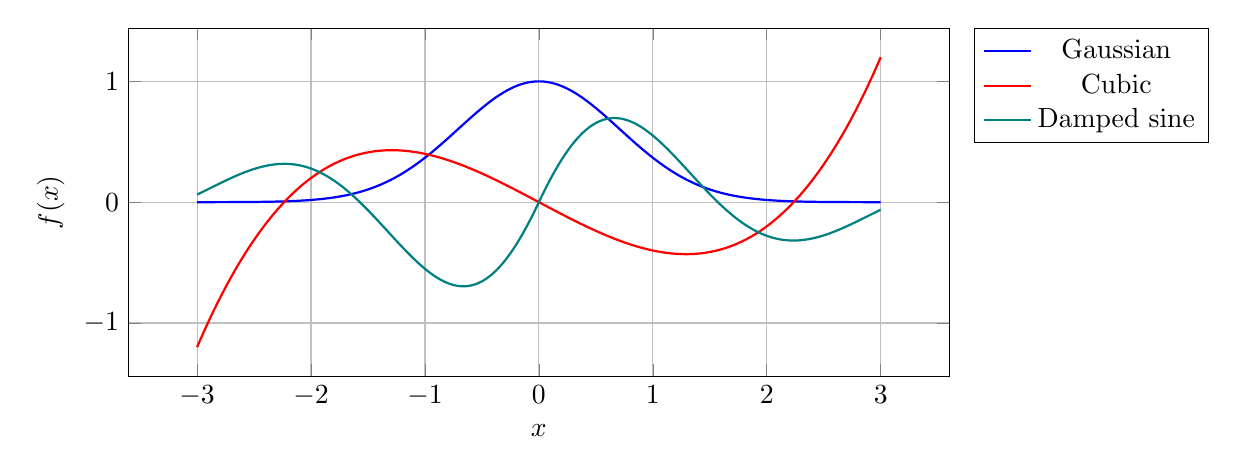
\begin{tikzpicture}
    \begin{axis}[width=12cm, height=6cm, xlabel=$x$, ylabel=$f(x)$, grid=both, legend pos=outer north east]
      \addplot[blue, thick, domain=-3:3, samples=200] {exp(-x^2)};
      \addplot[red, thick, domain=-3:3, samples=200] {x^3/10 - x/2};
      \addplot[teal, thick, domain=-3:3, samples=200] {sin(deg(2*x))*exp(-abs(x)/2)};
      \legend{Gaussian, Cubic, Damped sine}
    \end{axis}
  \end{tikzpicture}
  \caption{Three functions, 600 samples.}
\end{figure}

\begin{figure}[h]
  \centering
  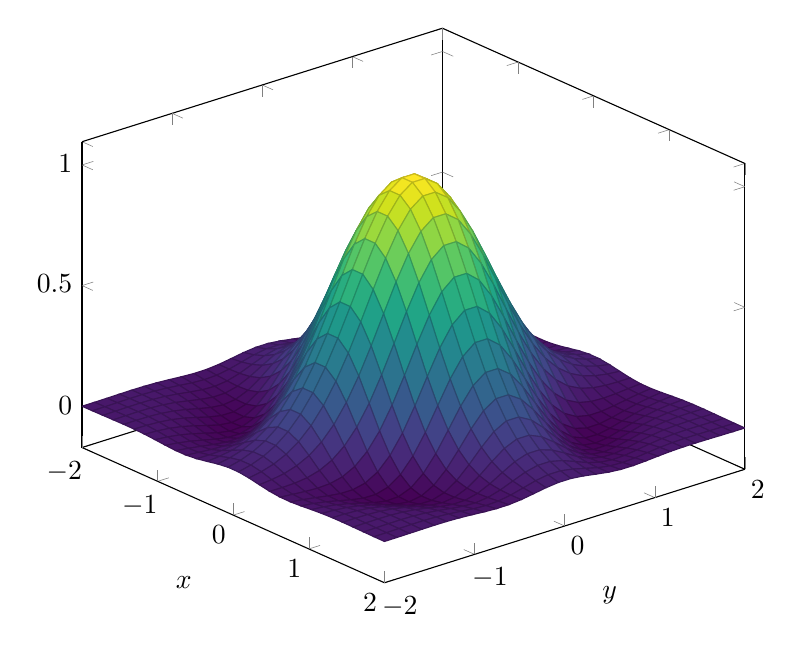
\begin{tikzpicture}
    \begin{axis}[view={50}{30}, width=10cm, colormap/viridis, xlabel=$x$, ylabel=$y$]
      \addplot3[surf, domain=-2:2, samples=30] {exp(-x^2-y^2)*cos(deg(2*x*y))};
    \end{axis}
  \end{tikzpicture}
  \caption{A surface of 900 facets.}
\end{figure}

\begin{figure}[h]
  \centering
  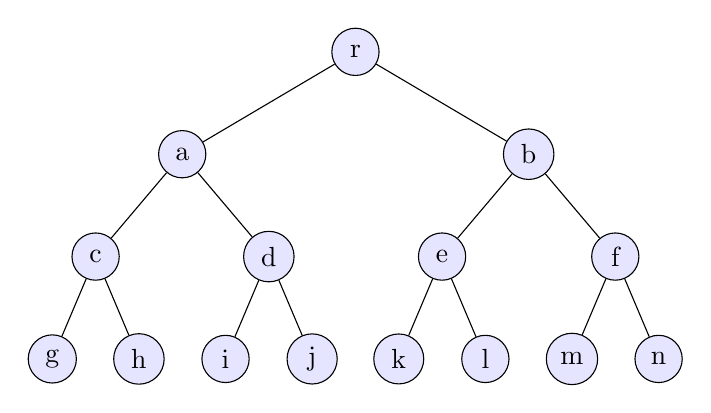
\begin{tikzpicture}[level distance=1.3cm, level 1/.style={sibling distance=4.4cm},
                      level 2/.style={sibling distance=2.2cm}, level 3/.style={sibling distance=1.1cm},
                      every node/.style={circle, draw, fill=blue!10, minimum size=6mm}]
    \node {r}
      child { node {a} child { node {c} child {node {g}} child {node {h}} } child { node {d} child {node {i}} child {node {j}} } }
      child { node {b} child { node {e} child {node {k}} child {node {l}} } child { node {f} child {node {m}} child {node {n}} } };
  \end{tikzpicture}
  \caption{A complete binary tree of depth three.}
\end{figure}

\begin{figure}[h]
  \centering
  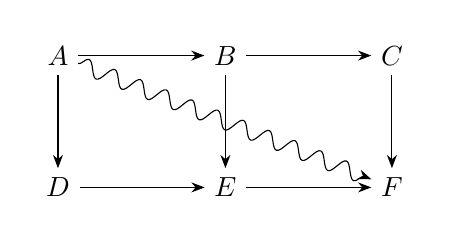
\begin{tikzpicture}
    \matrix (m) [matrix of math nodes, row sep=1.2cm, column sep=1.6cm] {
      A & B & C \\
      D & E & F \\
    };
    \foreach \from/\to in {1-1/1-2, 1-2/1-3, 2-1/2-2, 2-2/2-3, 1-1/2-1, 1-2/2-2, 1-3/2-3}
      \draw[-Stealth] (m-\from) -- (m-\to);
    \draw[-Stealth, decorate, decoration={snake, amplitude=1mm}] (m-1-1) -- (m-2-3);
  \end{tikzpicture}
  \caption{A commutative diagram with a decorated edge.}
\end{figure}

\begin{figure}[h]
  \centering
  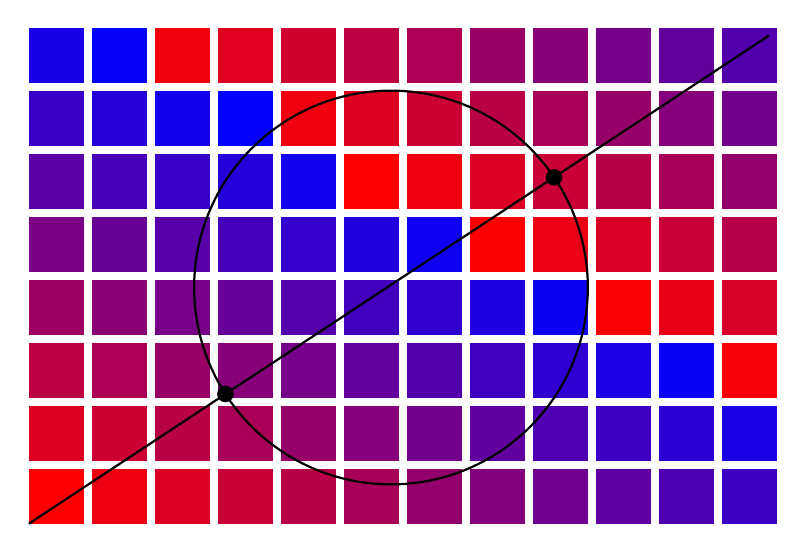
\begin{tikzpicture}
    \foreach \i in {0,...,11} {
      \foreach \j in {0,...,7} {
        \pgfmathsetmacro{\shade}{mod(\i*7+\j*13,100)}
        \fill[blue!\shade!red] (\i*0.8,\j*0.8) rectangle ++(0.7,0.7);
      }
    }
    \draw[name path=circle, thick] (4.6,3) circle (2.5);
    \draw[name path=line, thick] (0,0) -- (9.4,6.2);
    \fill[black, name intersections={of=circle and line, total=\t}]
      \foreach \k in {1,...,\t} {(intersection-\k) circle (3pt)};
  \end{tikzpicture}
  \caption{A 96-cell grid with computed colours and path intersections.}
\end{figure}

\begin{figure}[h]
  \centering
  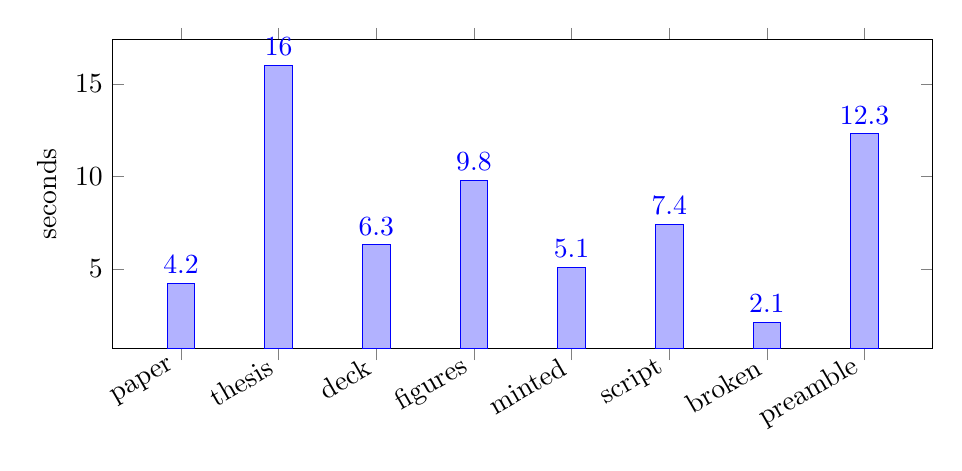
\begin{tikzpicture}
    \begin{axis}[ybar, width=12cm, height=5.5cm, symbolic x coords={paper,thesis,deck,figures,minted,script,broken,preamble},
                 xtick=data, x tick label style={rotate=30, anchor=east}, ylabel={seconds}, nodes near coords]
      \addplot coordinates {(paper,4.2) (thesis,16.0) (deck,6.3) (figures,9.8) (minted,5.1) (script,7.4) (broken,2.1) (preamble,12.3)};
    \end{axis}
  \end{tikzpicture}
  \caption{Cold build time per corpus document (illustrative).}
\end{figure}

\end{document}
